\documentclass[]{standalone}
\usepackage{amsmath}
\usepackage[utf8]{inputenc}
\usepackage[american]{circuitikz}
\usetikzlibrary{arrows,shapes,calc,positioning}

\begin{document}

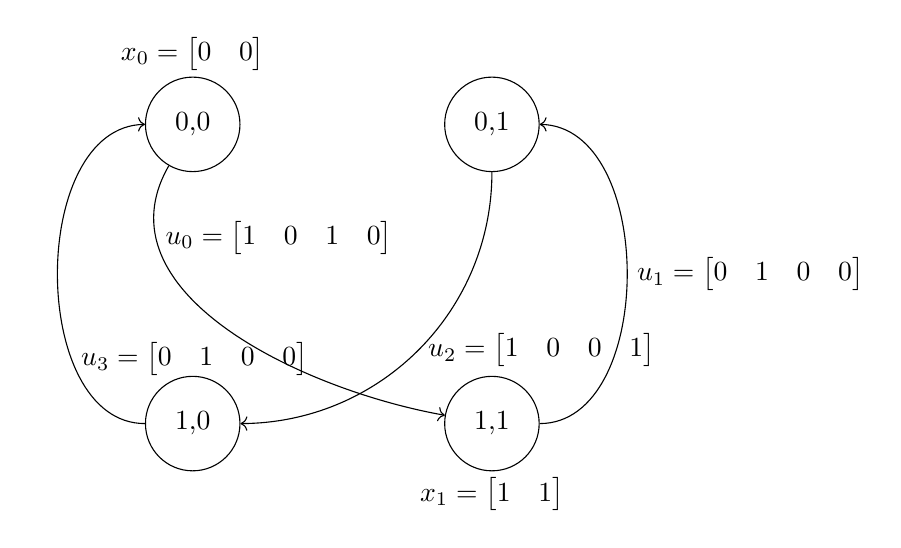
\begin{tikzpicture}[scale=1, node distance=38mm]
  \node[circle, draw, minimum height=12mm] (ab00) {0,0};
  \node[above of=ab00, node distance=9mm] {$x_0=\begin{bmatrix}0 & 0\end{bmatrix}$};
  \node[circle, draw, minimum height=12mm, right of=ab00] (ab01) {0,1};
  \node[circle, draw, minimum height=12mm, below of=ab01] (ab11) {1,1};
  \node[below of=ab11, node distance=9mm] {$x_1=\begin{bmatrix}1 & 1\end{bmatrix}$};
  \node[circle, draw, minimum height=12mm, left of=ab11] (ab10) {1,0};

  \draw[->] (ab00) to[out=-120, in=170] node[right, pos=0.2] {$u_0=\begin{bmatrix} 1 & 0 & 1 & 0 \end{bmatrix}$}  (ab11);
  \draw[->] (ab11) to[out=0, in=0] node[right] {$u_1=\begin{bmatrix} 0 & 1 & 0 & 0 \end{bmatrix}$}  (ab01);
  \draw[->] (ab01) to[out=-90, in=0] node[right] {$u_2=\begin{bmatrix} 1 & 0 & 0 & 1 \end{bmatrix}$}  (ab10);
  \draw[->] (ab10) to[out=-180, in=180, pos=0.3] node[right] {$u_3=\begin{bmatrix} 0 & 1 & 0 & 0 \end{bmatrix}$}  (ab00);
\end{tikzpicture}
\end{document}
